\documentclass[utf8,a4paper,nofonts]{ctexbook}

\usepackage{xcolor}
\usepackage{hyperref}
\usepackage{graphicx}

\usepackage{src/package/Listings}

\NewDocumentCommand\TODO{m}{\footnote{\textcolor{red}{TODO: #1}}}

\def\dif{\mathop{}\!\mathrm{d}}

\setCJKmainfont[Path=../fonts/,BoldFont=SourceHanSerifCN-Bold.otf,ItalicFont=SourceHanSerifCN-Bold.otf]{SourceHanSerifCN-Regular.otf}
\setCJKsansfont[Path=../fonts/,BoldFont=SourceHanSansCN-Bold.otf]{SourceHanSansCN-Regular.otf}
\setCJKmonofont[Path=../fonts/]{SourceHanSansCN-Regular.otf}

\title{Cookbook}
\author{周泓余\thanks{PeterlitsZo}}

\begin{document}

\maketitle

\tableofcontents
\newpage

\chapter{数学}

虽然我的确想要把所有笔记都记录在 Obsidian 中,但是数学相关的内容用 Obsidian 写起来还是太麻烦了。还是挪到这里吧。

\section{统计和概率学}

\subsection{正态分布}

我们说一个随机变量 $X$ 服从正态分布,那么我们记为 $X \sim N(\mu, \sigma^2)$。

这里的 $\mu$ 表示期望,$\sigma^2$ 表示方差。正态分布的概率密度函数为:

$$
f(x) = {1 \over \sqrt{2\pi}\sigma} \exp\left(-{(x - \mu)^2 \over 2\sigma^2}\right)
$$

我们将 $X \sim N(0, 1)$ 的随机变量称为标准正态分布。这个时候我们带入有概率密度函数如下:

$$
f(x) = {1 \over \sqrt{2\pi}} \exp\left(-{x^2 \over 2}\right)
$$

另外,对于 $X \sim N(\mu, \sigma^2)$ 而言,我们可以说 $Y = {X - \mu \over \sigma}$ 服从标准正态分布。

在 Rust 中,我们可以通过下面的方式来完成模拟(这里的 \verb|v| 即为一个正态分布的抽样):

\begin{lstlisting}
use rand_distr::{Distribution, Normal};

let normal = Normal::new(0.0, 1.0).unwrap();
let v = normal.sample(&mut rand::rng());
println!("{} is from a N(0, 1) distribution", v);
// 0.8033917292233297 is from a N(0, 1) distribution
\end{lstlisting}

在文档项目中的 \verb|playground| 目录下运行下面的命令即可:

\begin{lstlisting}
cargo run --bin 00_normal
\end{lstlisting}

\subsection{伊藤引理}
\label{ItosLemma}

[TODO]

\subsection{标准布朗运动}

我们这么定义标准布朗运动,对于定义在非负实数(时域)$t$ 上的连续随机过程 $\{B_t, t \ge 0\}$,满足以下条件:

\begin{itemize}
    \item $B(0) = 0$;
    \item 平稳性:对于所有 $0 < s < t$,增量 $B(t) - B(s)$ 符合均值为 $0$,方差为 $t - s$ 的正态分布。
    \item 独立增量:对于所有 $0 \le s < t < u < v$,增量 $B(t) - B(s)$ 和 $B(v) - B(u)$ 是独立的。
\end{itemize}

这个时候我们就说 $B(t)$ 是一个标准布朗运动。

在编程实现中,想要模拟连续的标准布朗运动是不现实且没有必要的,我们可以用离散的方式来模拟。
在 Rust 中,随机数可以通过 \verb|rand| 来生成,但是为了通过正态分布生成随机数,我们还需要使用 \verb|rand_distr|。
我们假设按照单位时间为 1s,那么中国股市的一天的交易时间就一共有 14400 个单位时间(对应 4 个小时)。
我们尝试循环 14400 次,每次都生成单位时间内对应的差 $\Delta B$,并且将其累加到 $B$ 上。
根据标准布朗运动的定义,我们很容易知道 $\Delta B$ 服从一个均值为 0,方差为 1 的标准正态分布(我们定义单位时间的长度就是 $1$)。
然后因为增量都是独立的,所以 $\Delta B$ 的求值和之前的求值无关,这是一个非常优良的特征。这使得下面的代码很容易实现:

\begin{lstlisting}
use rand_distr::{Distribution, Normal};

fn std_brownian_motion(steps: usize) -> Vec<f64> {
    let mut rng = rand::rng();

    let normal = Normal::new(0.0, 1.0).unwrap();
    let mut bm = vec![0.0];

    for _ in 0..steps {
        let v = normal.sample(&mut rng);
        bm.push(bm.last().unwrap() + v);
    }

    bm
}

std_brownian_motion(14400);
\end{lstlisting}

在文档项目中的 \verb|playground| 目录下运行如下命令即可:

\begin{lstlisting}
cargo run --bin 01_std_brownian_motion
\end{lstlisting}

在浏览器中,可以看到标准布朗运动的图像。如图 \ref{fig:stdBrownianMotion} 所示。

\begin{figure}[h]
    \centering
    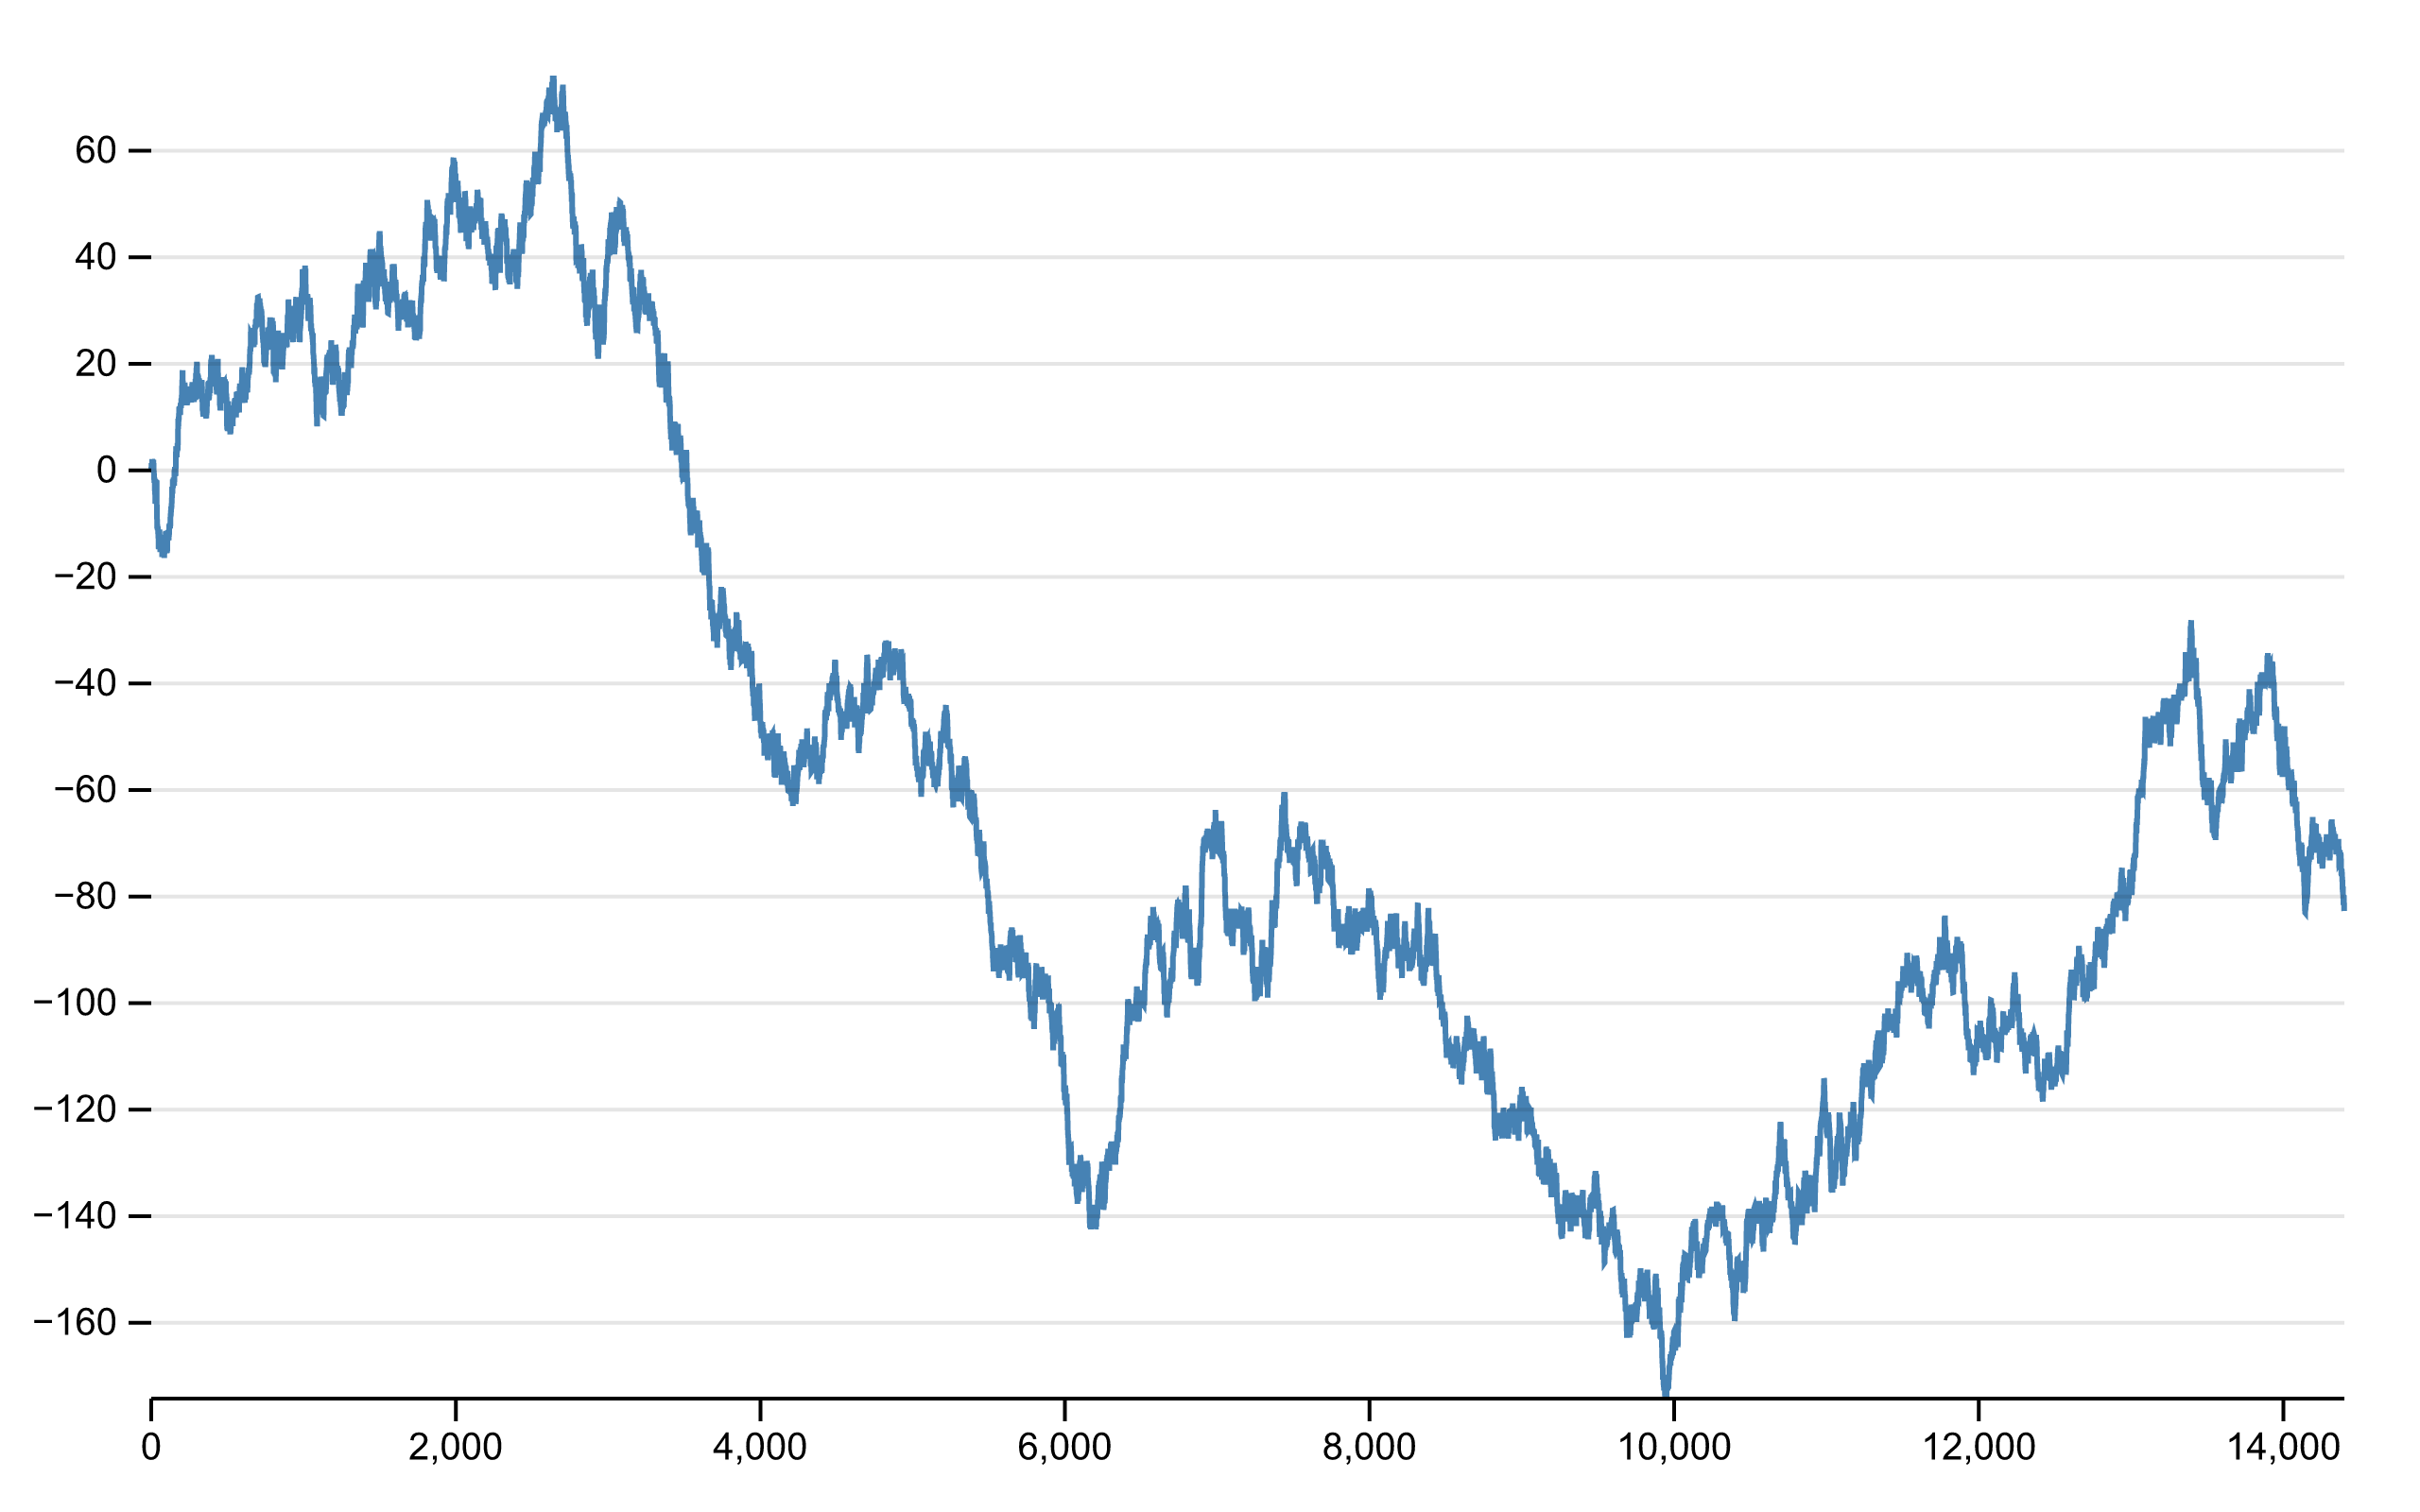
\includegraphics[width=0.8\textwidth]{src/static/00_std_brownian_motion.png}
    \caption{标准布朗运动}
    \label{fig:stdBrownianMotion}
\end{figure}

\subsection[几何布朗运动]{几何布朗运动\protect\footnotemark}
\footnotetext{见 \url{https://zhuanlan.zhihu.com/p/38293827}。}

我们可以在标准布朗运动 $B(t)$ 的基础上定义几何布朗运动。在定义之前,我们先定义有漂移的布朗运动 $X(t)$,它有:

$$
\dif{X(t)} = \mu \dif{t} + \sigma \dif{B(t)}
$$

我们知道 $B(t)$ 随机变量在 $t = 1$ 的期望为 $0$,而标准差为 $1$,经过偏移后,$X(t)$ 的期望和方差属性都有所变化。
这里 $\mu$ 被用于表示在单位时间内的期望增长率,而 $\sigma$ 被用于表示单位时间内的标准差。

在量化交易中,我们可以使用这个来描述收益率,而对于股票价格 $S(t)$ 而言,因为有 ${\dif{S(t)} \over S(t)} = \dif{X(t)}$。所以有:

$$
\dif{S(t)} = \mu S(t) \dif{t} + \sigma S(t) \dif{B(t)}
$$

通过伊藤引理 \ref{ItosLemma},我们可以得到:

$$
S(t) = S_0 \exp\left(\left(\mu - {\sigma^2 \over 2}\right)t + \sigma B(t)\right)
$$

我们可以使用 Rust 来对齐进行描述:

\begin{lstlisting}
use rand_distr::{Distribution, Normal};

fn geo_brownian_motion(steps: usize, mu: f64, sigma: f64, s0: f64) -> Vec<f64> {
    let mut rng = rand::rng();

    let normal = Normal::new(0.0, 1.0).unwrap();
    let mut bm = vec![s0];

    for _ in 0..steps {
        let z = normal.sample(&mut rng);
        let last_val = bm.last().unwrap();

        let drift = mu - 0.5 * sigma.powi(2);
        let diffusion = sigma * z;
        let new_val = last_val * (drift + diffusion).exp();

        bm.push(new_val);
    }

    bm
}
\end{lstlisting}

在 \verb|playground| 目录下运行如下命令即可:

\begin{lstlisting}
cargo run --bin 02_geo_brownian_motion
\end{lstlisting}

可以在浏览器中看到对应的几何布朗运动的图像。图 \ref{fig:geoBrownianMotion} 展示了几何布朗运动的一个例子。
(在这个图中,我们假定它为一个指数的日内曲线,其中年化收益率为 $8\%$,而一年的方差设置为 $10$)。

\begin{figure}[h]
    \centering
    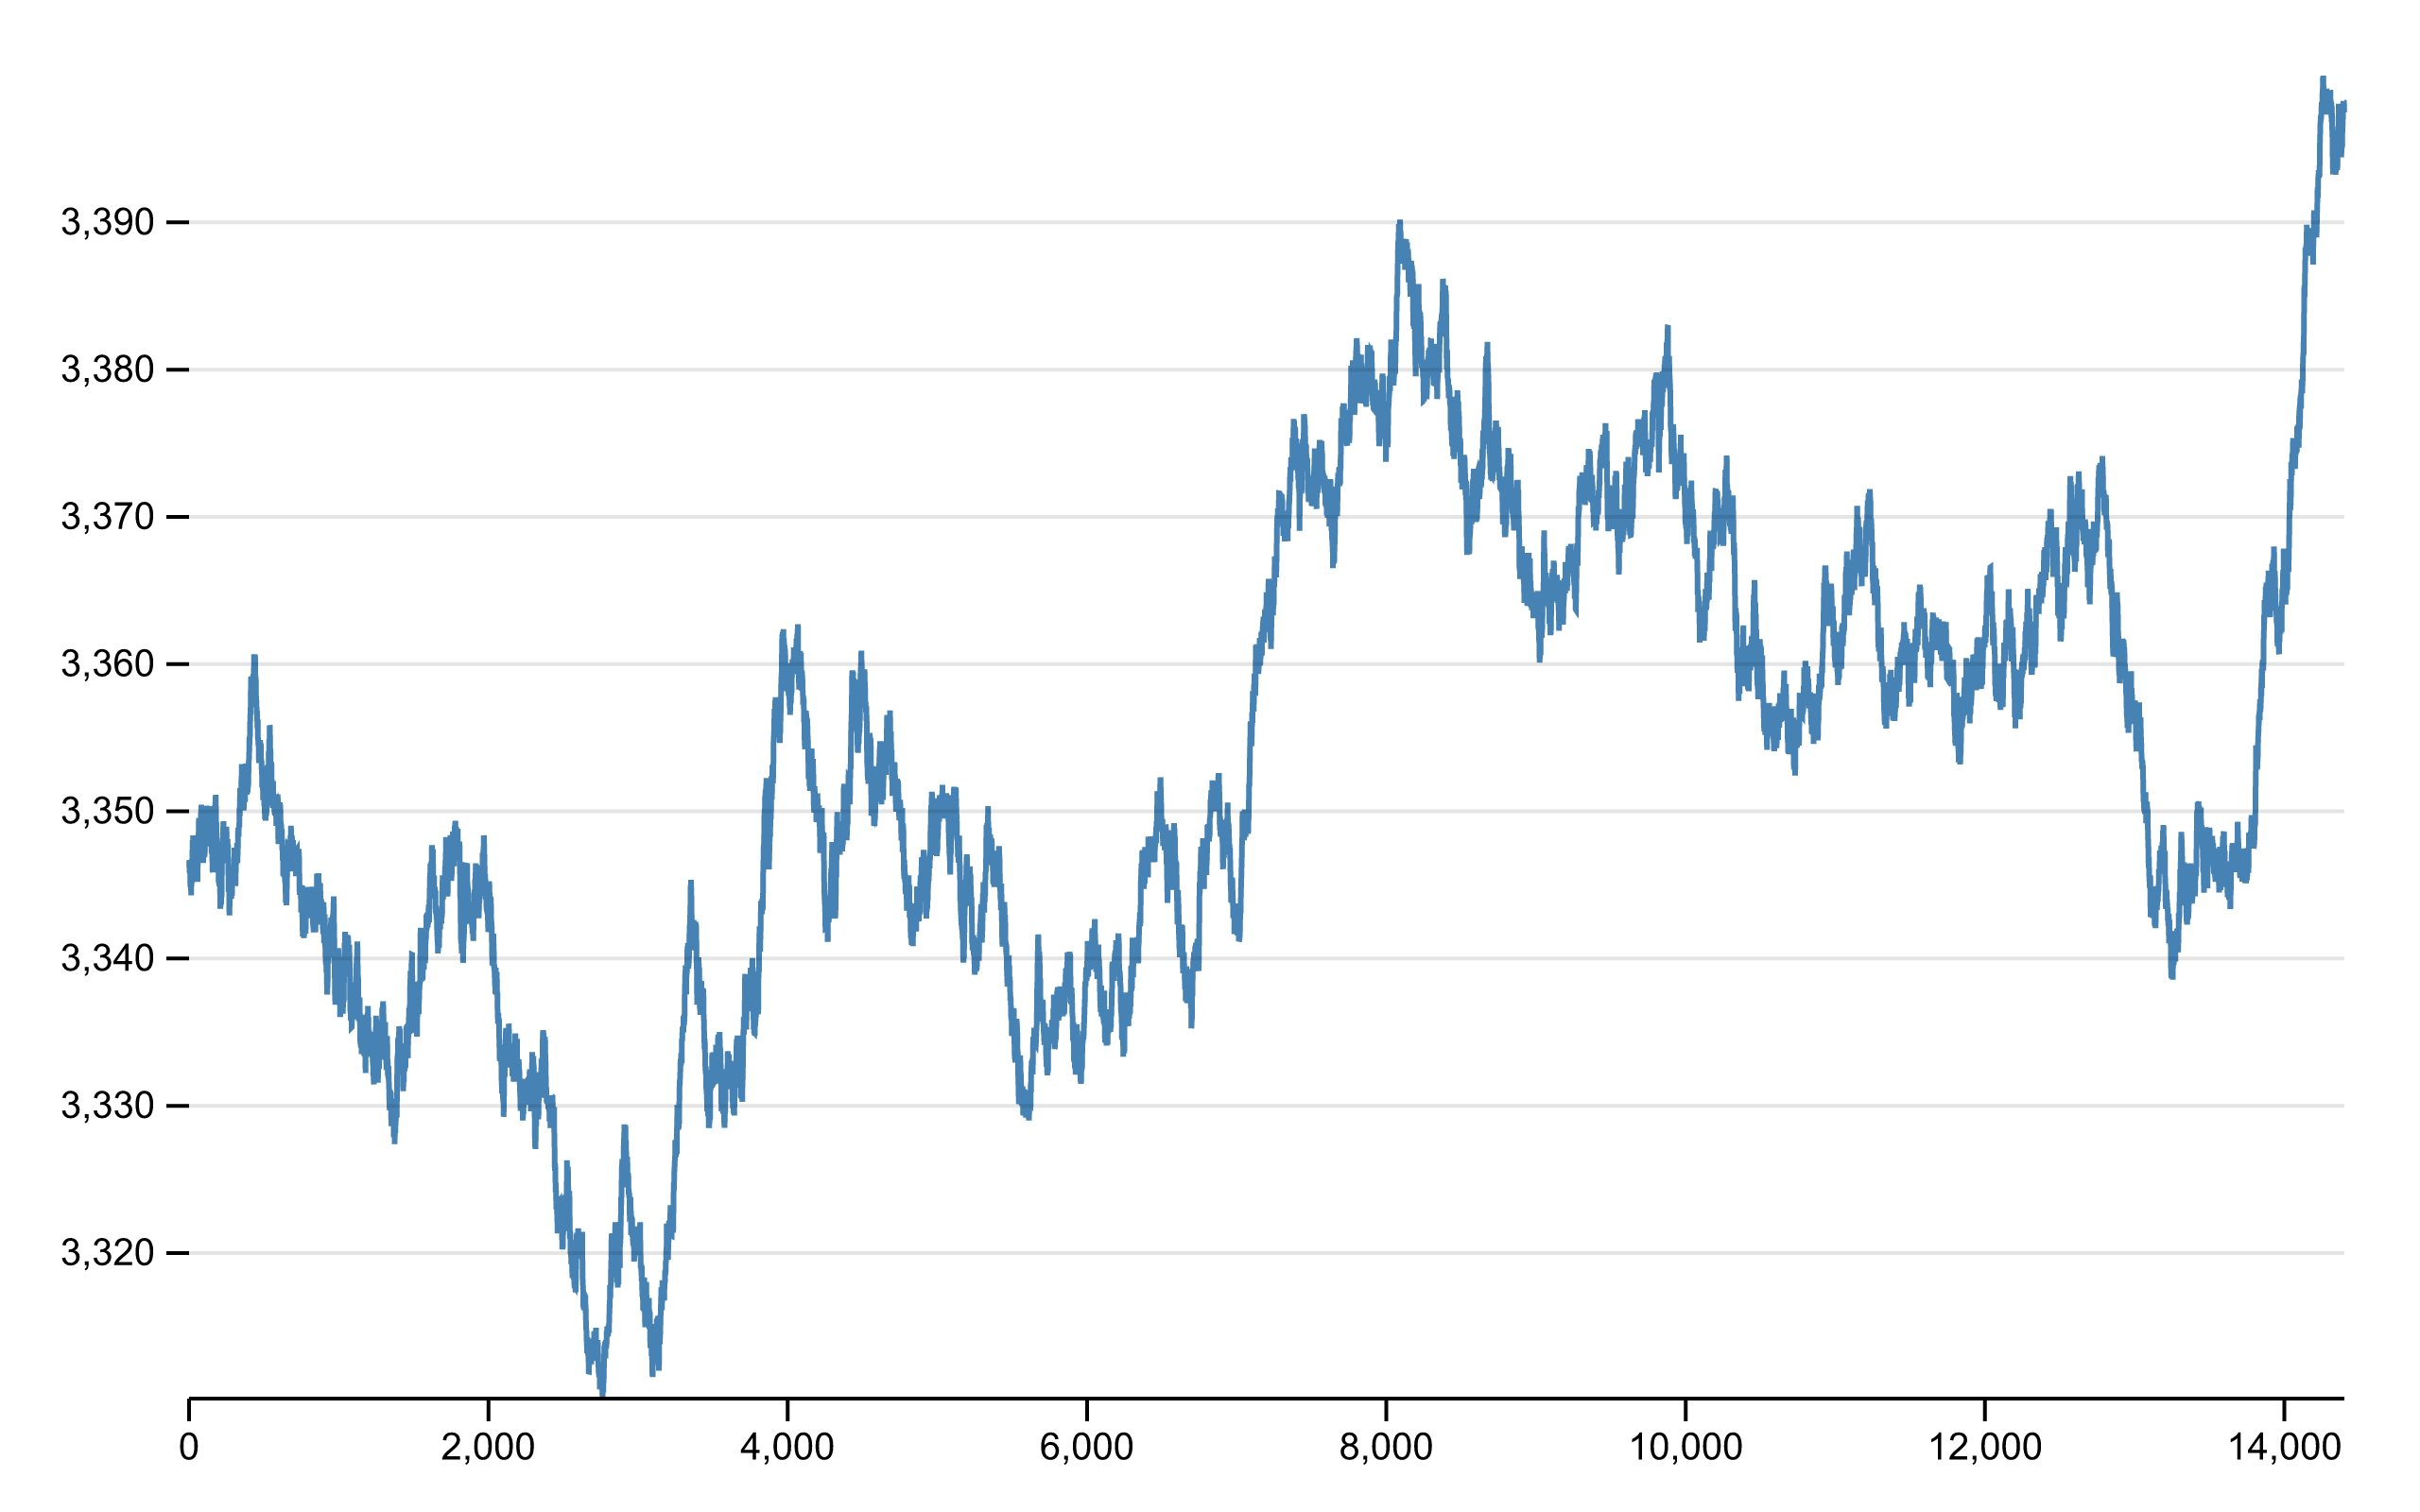
\includegraphics[width=0.8\textwidth]{src/static/01_geo_brownian_motion.png}
    \caption{几何布朗运动}
    \label{fig:geoBrownianMotion}
\end{figure}

\end{document}